\label{\part{\part{key}}}% EXEC_14 — Beamer compendium EJ-204 vs EJ-230
% SHiP Timing Detector Collaboration Meeting, 15–16 June 2026
% Clarified END/TOP notation, F1/F2 reading, L/R timing, and conservative interpretation of F2/F6/F7
% Compile: lualatex exec14_deck.tex && lualatex exec14_deck.tex
\documentclass[aspectratio=169,9pt]{beamer}

% ── Theme ─────────────────────────────────────────────────────────────────────
\usetheme{Madrid}
\usecolortheme{default}
\setbeamertemplate{navigation symbols}{}
\setbeamerfont{frametitle}{size=\normalsize,series=\bfseries}
\setbeamerfont{framesubtitle}{size=\small}

% ── Fonts (LuaLaTeX) ─────────────────────────────────────────────────────────
\usepackage{fontspec}
\setsansfont{DejaVu Sans}[Scale=0.93]
\setmonofont{DejaVu Sans Mono}[Scale=0.85]

% ── Packages ──────────────────────────────────────────────────────────────────
\usepackage{graphicx}
\usepackage{booktabs}
\usepackage{xcolor}
\usepackage{siunitx}
\sisetup{separate-uncertainty=true}
\usepackage{tikz}
\usetikzlibrary{arrows.meta}

\graphicspath{{outputs/}}

% ── Colors ────────────────────────────────────────────────────────────────────
\definecolor{ej204col}{HTML}{1f78b4}
\definecolor{ej230col}{HTML}{e31a1c}
\definecolor{okgreen}{HTML}{2ca02c}
\definecolor{pendgold}{HTML}{d4a017}

% ── Metadata ──────────────────────────────────────────────────────────────────
\title[EJ-204 vs EJ-230 — SHiP Timing]{%
  Optical Simulation of Scintillator Bars\\
  \large EJ-204 vs EJ-230 for the SHiP Timing Detector}
\author[R.~Ríos / G.~Vásquez]{%
  René Ríos \and Gerardo Vásquez}
\institute[SHiP Timing]{SHiP Collaboration — Timing Detector Group}
\date{15--16 June 2026}

% ══════════════════════════════════════════════════════════════════════════════
\begin{document}

\begin{frame}[plain]
  \titlepage
\end{frame}

\begin{frame}{Contents}
  \tableofcontents
\end{frame}

% ══════════════════════════════════════════════════════════════════════════════
\section{Setup and geometry}

\begin{frame}{Bar geometry and SiPM readout}
  \begin{columns}[T]
    \begin{column}{0.50\textwidth}
      \textbf{Scintillator bar (GEANT4):}
      \begin{itemize}
        \item Active length: \SI{1400}{\mm} ($\pm700$\,mm along $x$)
        \item Coating: reflective Mylar
        \item $v_\text{eff}\approx277$\,mm/ns (nominal axial average)
        \item[$\hookrightarrow$] {\footnotesize ToF onset measures $v_\text{eff}^\text{onset}\approx292$\,mm/ns
              ($+5\%$): set by the most direct rays, not the mean path (see QA-1c)}
        \item Two materials compared in parallel:\\
              \textcolor{ej204col}{\textbf{EJ-204}} vs
              \textcolor{ej230col}{\textbf{EJ-230}}
      \end{itemize}
      \vspace{0.2em}
      \textbf{End SiPMs (primary timing):}
      \begin{itemize}
        \item 16 SiPMs total (IDs 0–15)
        \item END\_LEFT: IDs 0–7 at $x=-700$\,mm
        \item END\_RIGHT: IDs 8–15 at $x=+700$\,mm
        \item Timing estimator: \textbf{SUM4} (fixed id$/\!/$4 clusters, earliest-of-two, leading-edge $\geq4$\,PE)
      \end{itemize}
    \end{column}
    \begin{column}{0.48\textwidth}
      \textbf{Top SiPMs (veto / tracking):}
      \begin{itemize}
        \item 70 SiPMs, single row at $Y=+30.25$\,mm
        \item TOP\_LEFT: IDs 16–50 / TOP\_RIGHT: 51–85
        \item Pitch: \SI{20}{\mm} in $X$; central gap \SI{24}{\mm}
      \end{itemize}
      \vspace{0.3em}
      \textbf{GEANT4 statistics:}
      \begin{center}
        \small
        \begin{tabular}{lrr}
          \toprule
          Dataset & Events & Positions \\
          \midrule
          EJ-204 End & 2000/pos & 31 \\
          EJ-230 End & 2000/pos & 31 \\
          EJ-204 EndTop & 2000/pos & 31 \\
          \bottomrule
        \end{tabular}\\[0.2em]
        {\footnotesize Positions: $x = 0, \pm50, \ldots, \pm690$\,mm}
      \end{center}
    \end{column}
  \end{columns}
  \vspace{-0.4em}
  \begin{beamercolorbox}[rounded=true,sep=0.45em,wd=\textwidth]{block body}
    {\scriptsize \textbf{Notation used below:} \textbf{END} = END\_LEFT $\cup$ END\_RIGHT
    (all IDs 0--15). ``Left/right column'' refers only to slide layout; physical sides are
    always written END\_LEFT or END\_RIGHT.}
  \end{beamercolorbox}
\end{frame}

% ══════════════════════════════════════════════════════════════════════════════
\section{Photon arrival-time profile — F1}

\begin{frame}{F1: Relative arrival time $t_\text{rel}$ — central position $x=0$}
  \framesubtitle{%
    \textcolor{ej204col}{\textbf{EJ-204}} (left \emph{column}) vs
    \textcolor{ej230col}{\textbf{EJ-230}} (right \emph{column}) —
    each material pools \textbf{both physical END faces}}
  \begin{center}
    \colorbox{yellow!16}{\parbox{0.94\textwidth}{\centering\scriptsize
      Here \textbf{END = END\_LEFT $\cup$ END\_RIGHT} (SiPM IDs 0--15).
      ``Left/right'' above describes the page columns, not the detector ends.}}
  \end{center}
  \vspace{-0.35em}
  \begin{columns}[c]
    \begin{column}{0.49\textwidth}
      \centering
      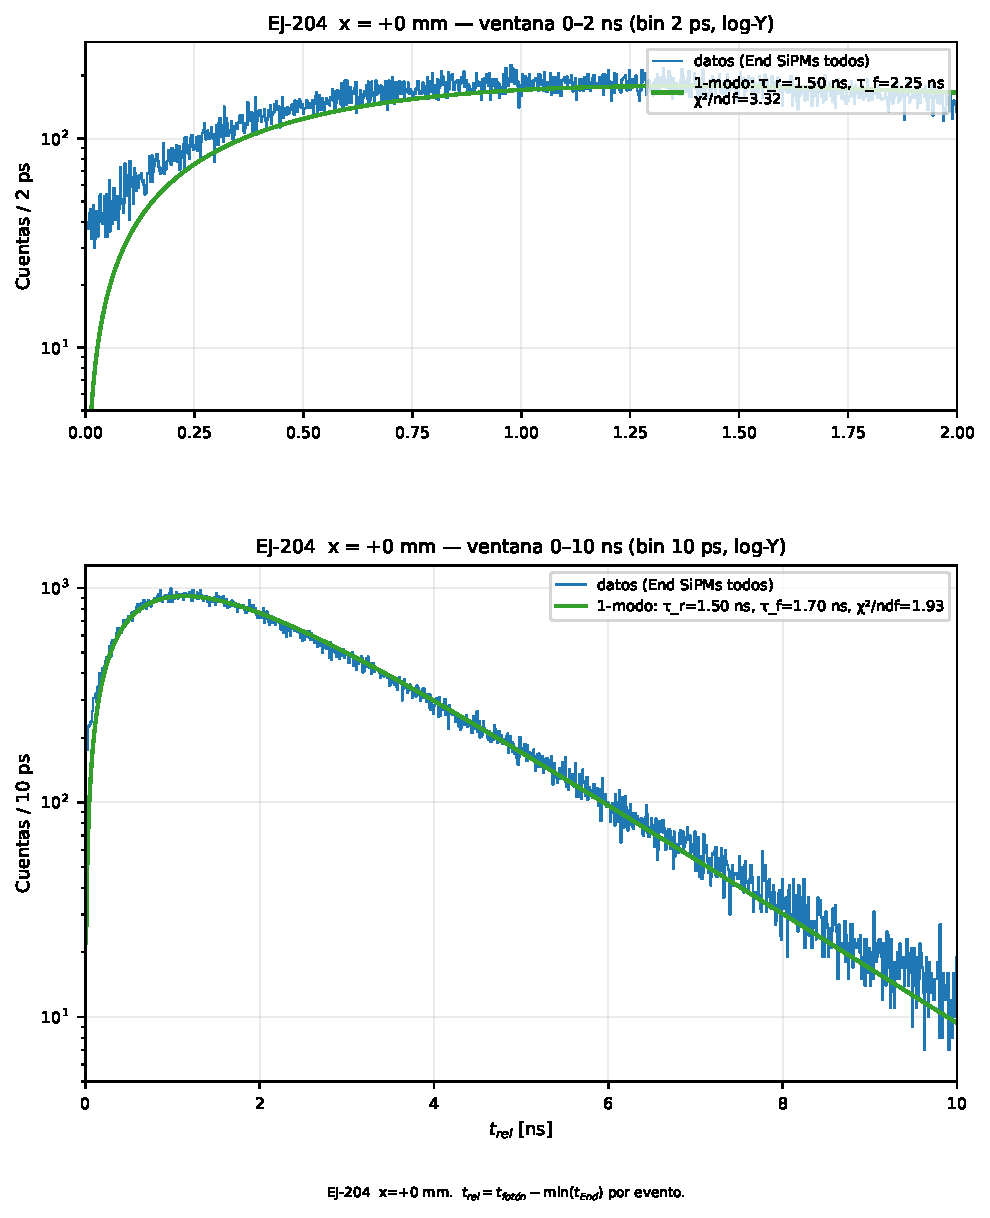
\includegraphics[height=0.53\textheight,keepaspectratio]{fig01a.pdf}
    \end{column}
    \begin{column}{0.49\textwidth}
      \centering
      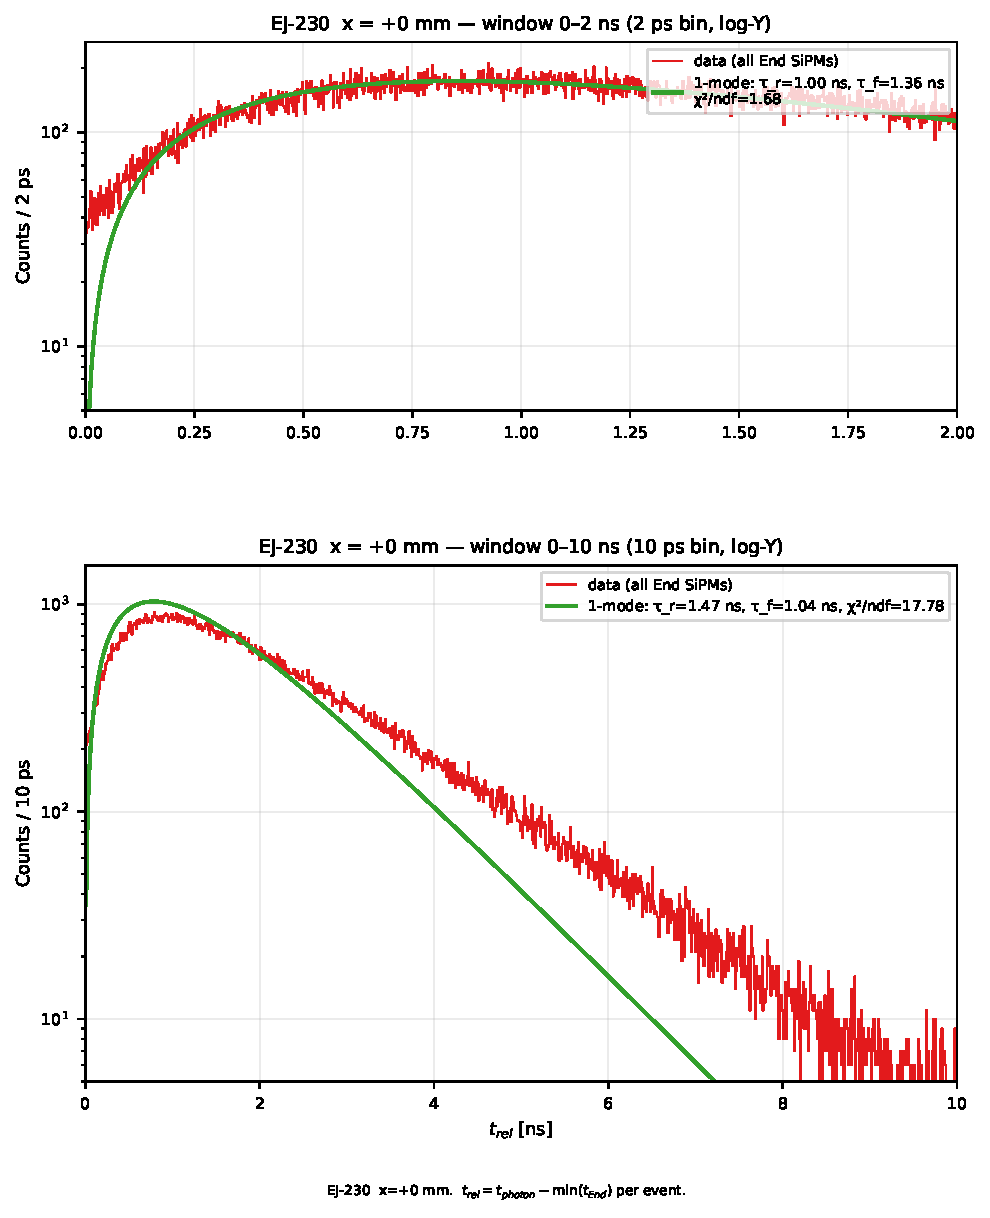
\includegraphics[height=0.53\textheight,keepaspectratio]{fig01d.pdf}
    \end{column}
  \end{columns}
  \vspace{-0.15em}
  \begin{center}
    {\scriptsize
      For event $e$: $t_{0,\mathrm{END}}^{(e)}=\min_{h:\,\mathrm{ID}(h)=0\ldots15}t_h$;
      every hit on either END face enters as $t_\text{rel}=t_h-t_{0,\mathrm{END}}^{(e)}$.\\[-0.05em]
      At $x=0$, either physical end can provide the first hit.
      EJ-204: $\tau_r=1.50$\,ns, $\tau_f=1.70$\,ns ($\chi^2/\text{ndf}=1.93$).\quad
      EJ-230: $\tau_r=1.47$\,ns, $\tau_f=1.04$\,ns ($\chi^2/\text{ndf}=17.8$).\\[-0.05em]
      \textit{These fitted $\tau$ describe an arrival profile
      (emission $\otimes$ propagation $\otimes$ first-hit referencing), not datasheet constants.}
      EJ-230's central tail cannot be a left--right ToF effect.}
  \end{center}
\end{frame}

\begin{frame}{F1: Relative arrival time $t_\text{rel}$ — edge position $x=+690$\,mm}
  \framesubtitle{Both END faces are pooled: END\_RIGHT is near, END\_LEFT is far}
  \begin{columns}[c]
    \begin{column}{0.49\textwidth}
      \centering
      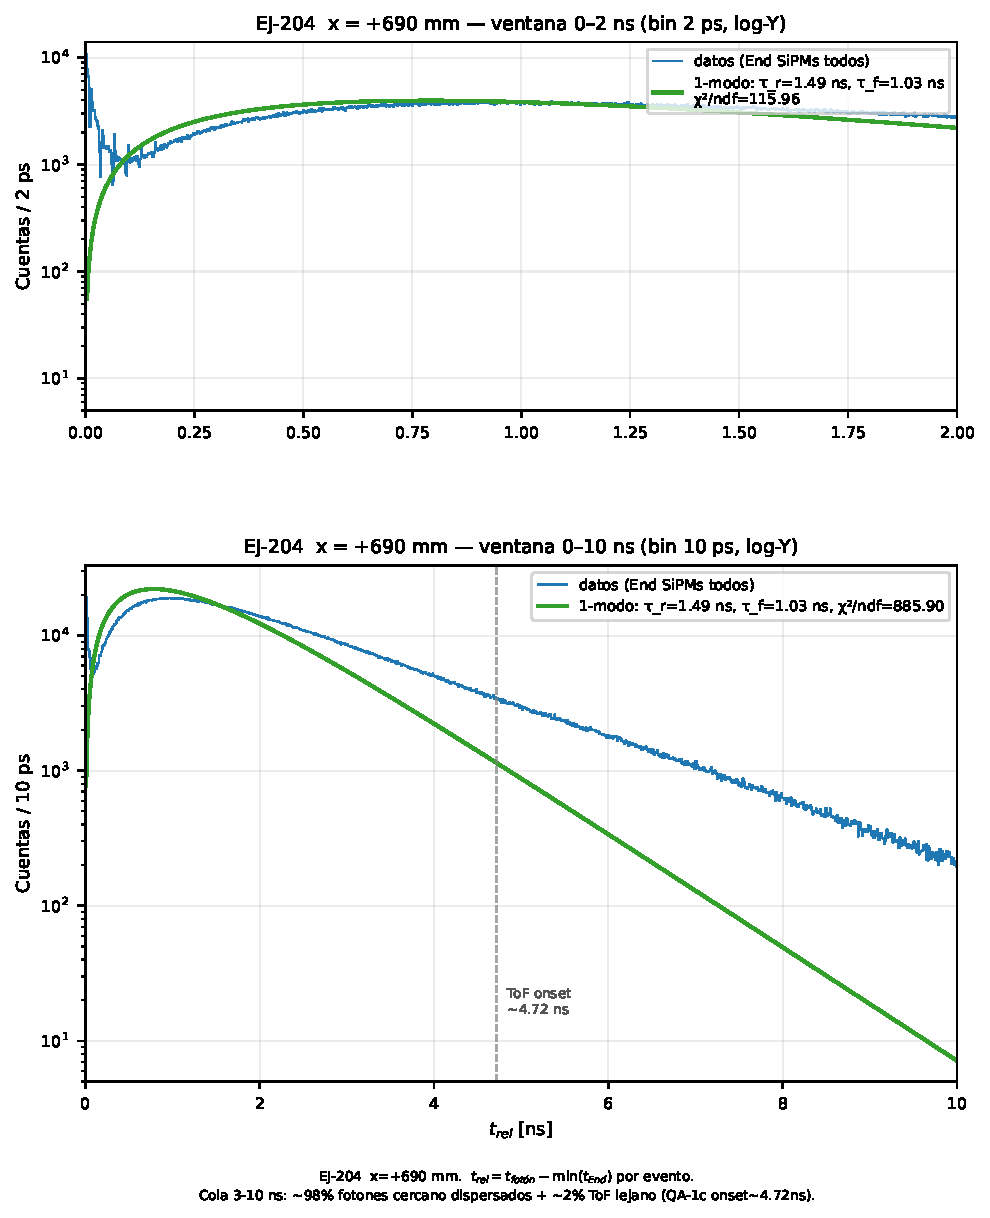
\includegraphics[height=0.66\textheight,keepaspectratio]{fig01c.pdf}
    \end{column}
    \begin{column}{0.49\textwidth}
      \centering
      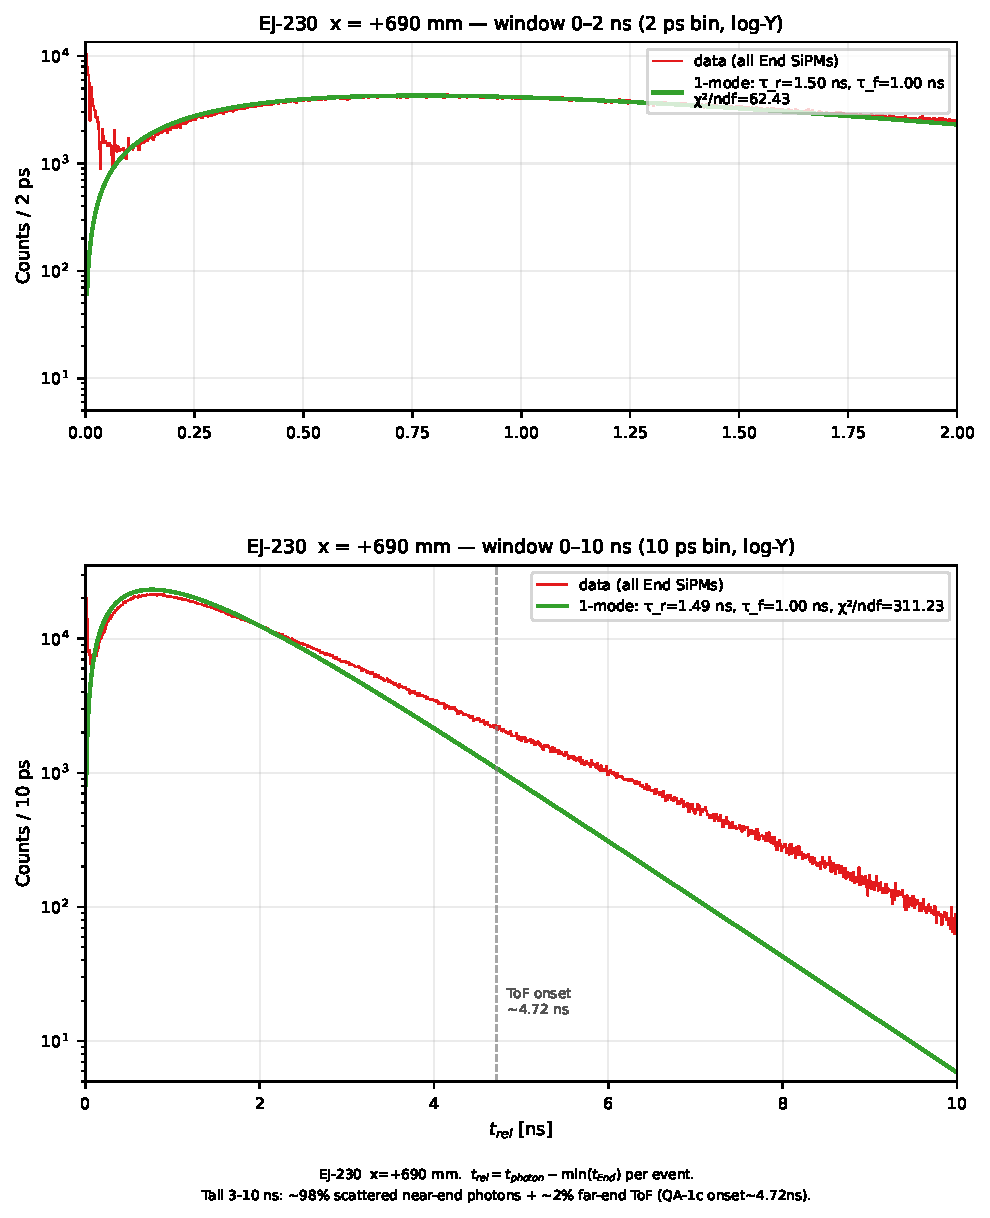
\includegraphics[height=0.66\textheight,keepaspectratio]{fig01f.pdf}
    \end{column}
  \end{columns}
  \vspace{-0.1em}
  \begin{center}
    {\scriptsize
      The early population is dominated by the nearby END\_RIGHT; the far END\_LEFT
      starts contributing at $t_\text{rel}\simeq4.7$\,ns. Both populations are superposed in F1.\\[-0.05em]
      A 1-mode fit therefore fails ($\chi^2/\text{ndf}=886$ for EJ-204 and $721$ for EJ-230).
      The late onset is geometric ToF, not evidence by itself for slow scintillation.}
  \end{center}
\end{frame}

% ══════════════════════════════════════════════════════════════════════════════
\section{Geometric time-of-flight — QA-1c}

% ── NEW SLIDE: ToF diagram ───────────────────────────────────────────────────
\begin{frame}{Why a second component appears at the edge — geometric time-of-flight}
  \begin{center}
  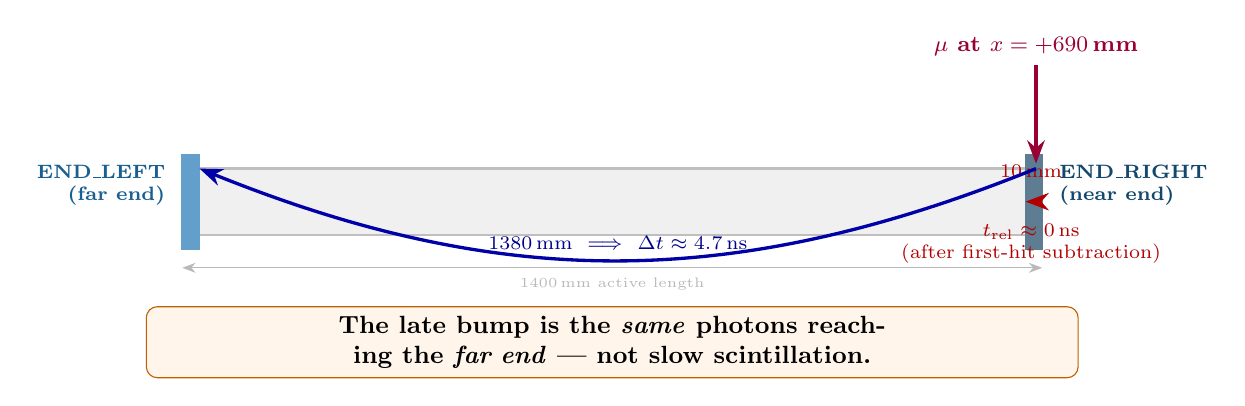
\begin{tikzpicture}[x=0.78cm, y=1.05cm, >=Stealth]

    % ── Bar body ──────────────────────────────────────────────────────────────
    \fill[gray!12] (-7,-0.40) rectangle (7,0.40);
    \draw[thick, gray!50] (-7,-0.40) rectangle (7,0.40);

    % ── END_LEFT SiPM (far end at x=-700 mm) ─────────────────────────────────
    \fill[ej204col!70] (-7.02,-0.58) rectangle (-6.72,0.58);
    \node[left, font=\scriptsize\bfseries, text=ej204col!80!black, align=right]
        at (-7.12, 0.20) {END\_LEFT\\(far end)};

    % ── END_RIGHT SiPM (near end at x=+700 mm) ───────────────────────────────
    \fill[ej204col!35!gray] (6.72,-0.58) rectangle (7.02,0.58);
    \node[right, font=\scriptsize\bfseries, text=ej204col!60!black, align=left]
        at (7.12, 0.20) {END\_RIGHT\\(near end)};

    % ── Muon at x=+690 mm (≈ +6.9 units) ────────────────────────────────────
    \draw[very thick, purple!80!black, ->] (6.90,1.65) -- (6.90,0.46);
    \node[above, font=\footnotesize\bfseries, text=purple!80!black]
        at (6.90,1.65) {$\mu$\ at\ $x=+690$\,mm};

    % ── Short path to near end (10 mm, ~0 ns) ────────────────────────────────
    \draw[very thick, red!70!black, ->] (6.90, 0.0) -- (6.73, 0.0);
    \node[above, font=\scriptsize, text=red!70!black] at (6.82, 0.18) {10\,mm};
    \node[below, font=\scriptsize, text=red!70!black, align=center] at (6.82,-0.15) {$t_\text{rel}\approx0$\,ns\\(after first-hit subtraction)};

    % ── Long path to far end (1380 mm, ~4.7 ns) — curved arc above bar ───────
    \draw[very thick, blue!65!black, ->]
        (6.90, 0.40) to[bend left=22]
        node[above, pos=0.50, font=\scriptsize, text=blue!55!black]
        {1380\,mm \ $\Longrightarrow$ \ $\Delta t \approx 4.7$\,ns}
        (-6.72, 0.40);

    % ── Bar length annotation ─────────────────────────────────────────────────
    \draw[<->, gray!55, thin] (-7,-0.80) -- (7,-0.80);
    \node[below, gray!55, font=\tiny] at (0,-0.80) {1400\,mm active length};

    % ── Key message ──────────────────────────────────────────────────────────
    \node[draw=orange!75!black, fill=orange!8, rounded corners=4pt,
          text width=11.6cm, align=center, font=\small\bfseries]
        at (0,-1.70)
        {The late bump is the \emph{same} photons reaching the \emph{far end} —
         not slow scintillation.};

  \end{tikzpicture}
  \end{center}
\end{frame}

\begin{frame}{QA-1c: Second F1 component confirmed as geometric ToF}
  \begin{columns}[c]
    \begin{column}{0.63\textwidth}
      \centering
      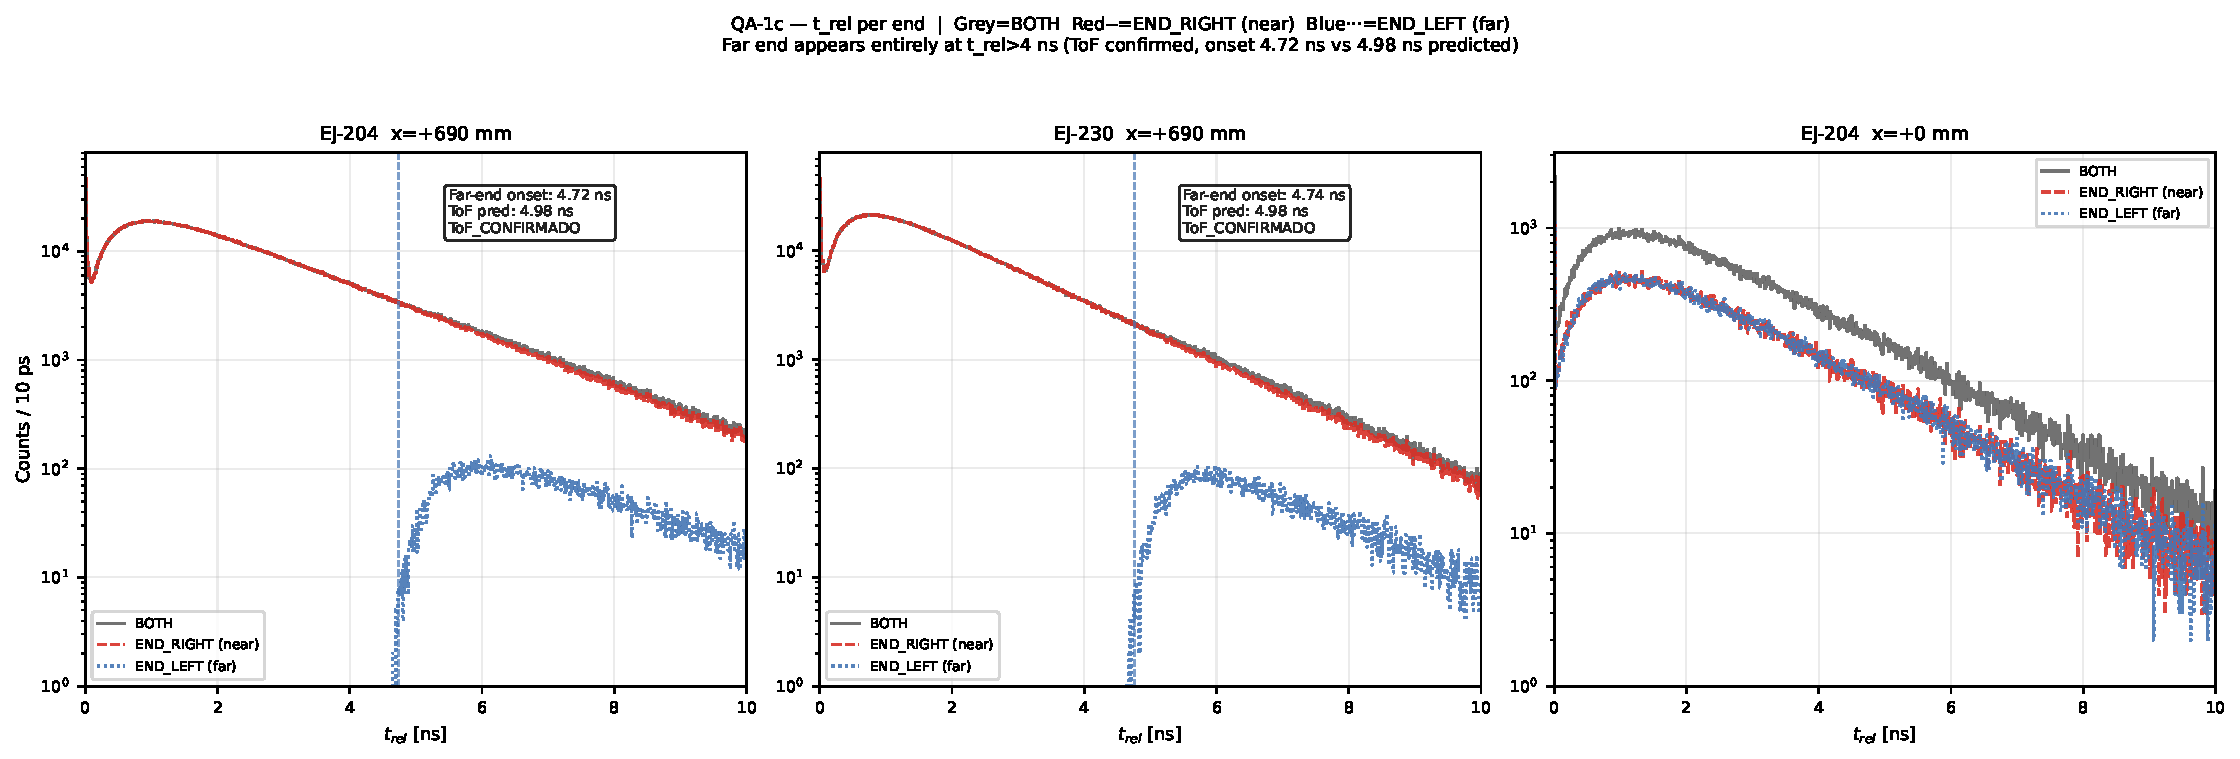
\includegraphics[width=\textwidth,keepaspectratio]{fig01_tof_probe_vis.pdf}
    \end{column}
    \begin{column}{0.35\textwidth}
      \textbf{ToF prediction ($x=+690$\,mm):}
      \[
        \Delta t_\text{pred} = \frac{1380\,\text{mm}}{277\,\text{mm/ns}}
        \approx 4.98\,\text{ns}
      \]

      \textbf{Measured onset (far end):}
      \begin{itemize}
        \item \textcolor{ej204col}{EJ-204}: $4.72$\,ns \hfill $(-5.3\%)$
        \item \textcolor{ej230col}{EJ-230}: $4.74$\,ns \hfill $(-4.9\%)$
      \end{itemize}

      \vspace{0.4em}
      \textbf{Verdict:}\\
      \textcolor{okgreen}{\textbf{ToF\_CONFIRMED}}\\[0.3em]
      {\footnotesize
        The $-5\%$ offset reflects $v_\text{eff}^\text{onset}\approx292$\,mm/ns
        — the fastest (most direct) optical rays arrive first,
        pulling the onset earlier than the mean-path prediction.}
    \end{column}
  \end{columns}
  \vspace{-0.15em}
  \begin{center}
    {\scriptsize \textbf{BOTH} is the union of photon hits from END\_LEFT and END\_RIGHT
    (grey $=$ red + blue bin by bin), not a coincidence time.
    The labels near/far apply to $x=+690$\,mm; at $x=0$ neither side is geometrically near or far.}
  \end{center}
\end{frame}

% ══════════════════════════════════════════════════════════════════════════════
\section{Spatial hit distribution — F3}

\begin{frame}{F3: Spatial distribution of photon impacts on SiPMs}
  \framesubtitle{Single representative event — EJ-204 (EJ-230 qualitatively identical)}
  \begin{columns}[c]
    \begin{column}{0.49\textwidth}
      \centering
      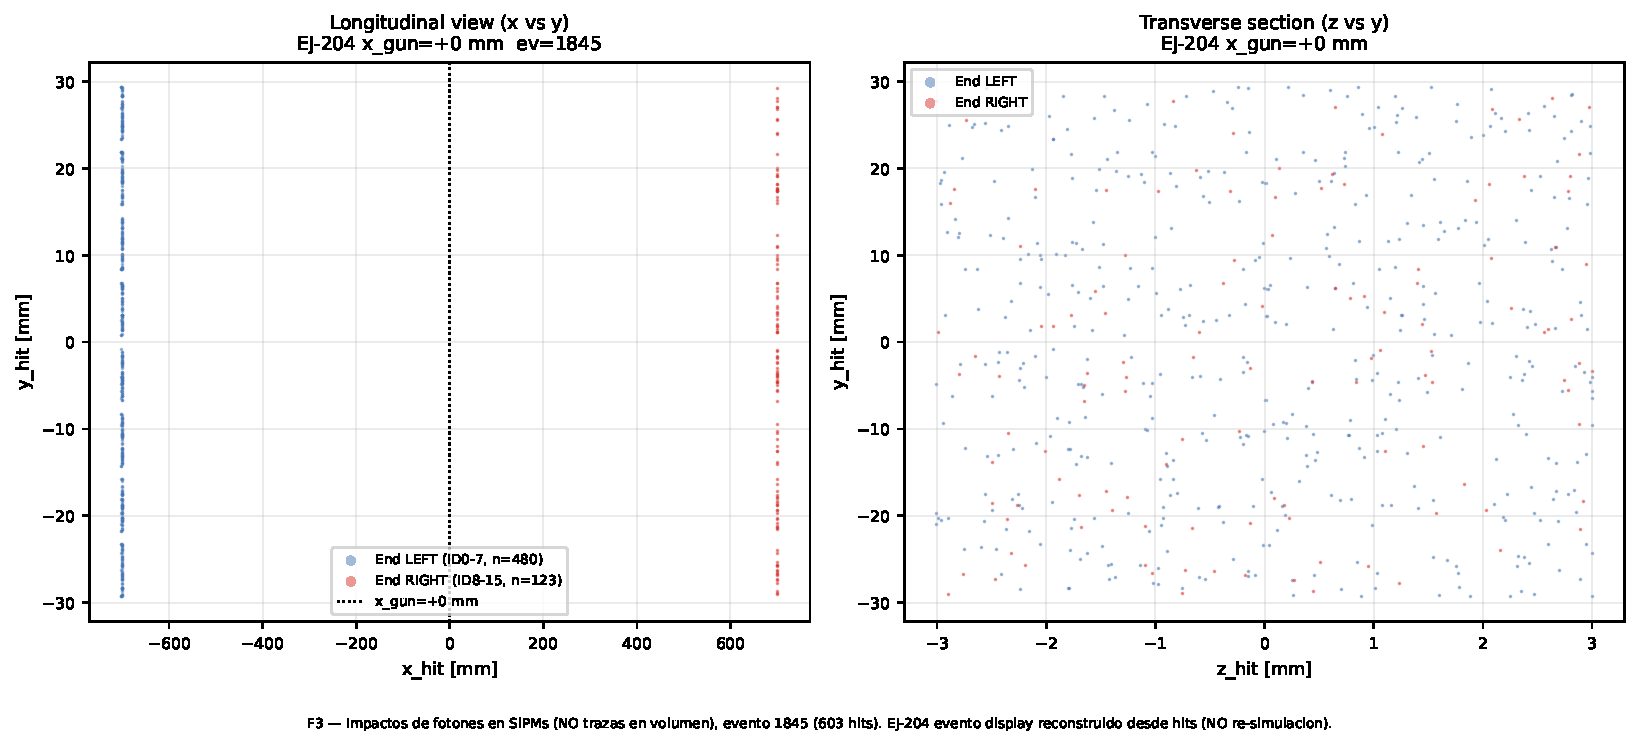
\includegraphics[width=\textwidth,keepaspectratio]{fig03a.pdf}\\
      {\footnotesize $x_\text{gun}=0$\,mm — both ends populated; this single event is not count-symmetric}
    \end{column}
    \begin{column}{0.49\textwidth}
      \centering
      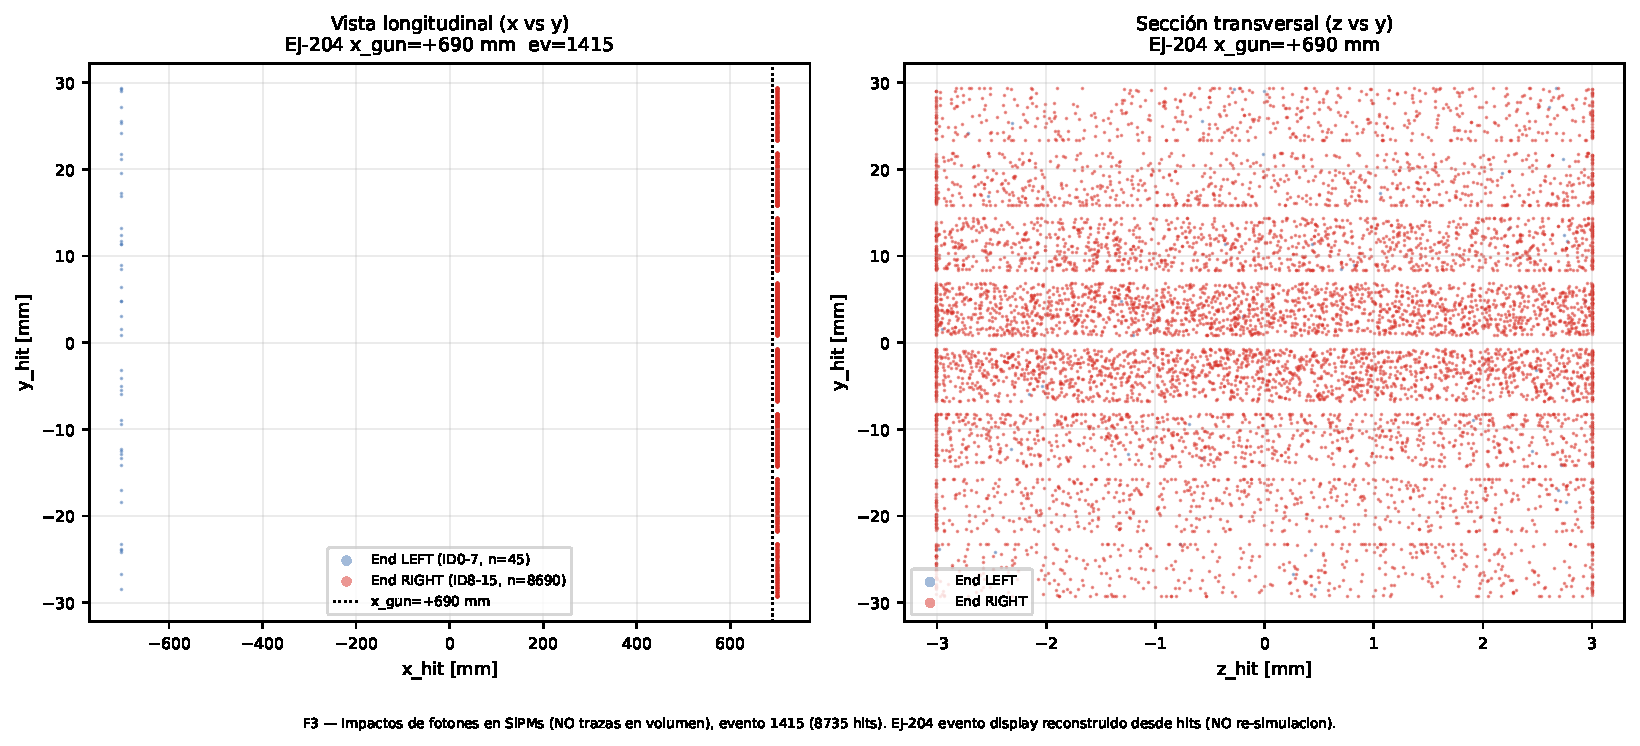
\includegraphics[width=\textwidth,keepaspectratio]{fig03b.pdf}\\
      {\footnotesize $x_\text{gun}=+690$\,mm — collapse toward END\_RIGHT}
    \end{column}
  \end{columns}
  \vspace{0.2em}
  {\footnotesize
    \textit{Note:} Points are \emph{photon impacts on the SiPM window}
    (NOT trajectories inside the scintillator volume). This is an endpoint map, not a ray-tracing view.
    Reconstructed from \texttt{x\_mm}/\texttt{y\_mm}/\texttt{z\_mm} ROOT branches — no re-simulation.}
\end{frame}

% ══════════════════════════════════════════════════════════════════════════════
\section{$\sigma_t$ vs $N_{pe}$ and Top profiles — F2, F4}

\begin{frame}{F2: $\sigma_t$ vs $N_{pe}$ — both END faces, analyzed separately}
  \framesubtitle{$N_L$: END\_LEFT (IDs 0--7), $N_R$: END\_RIGHT (IDs 8--15);
    fit variable $N_\text{weak}=\min(N_L,N_R)$}
  \begin{columns}[c]
    \begin{column}{0.48\textwidth}
      \centering
      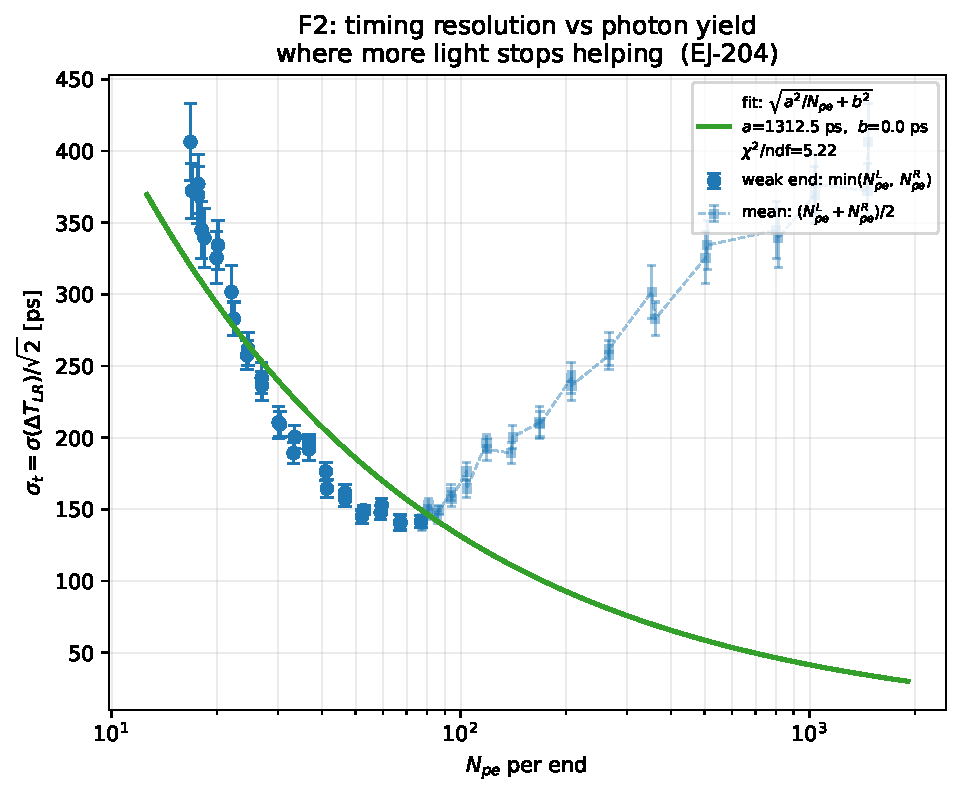
\includegraphics[width=0.90\textwidth,keepaspectratio]{fig02a.pdf}
    \end{column}
    \begin{column}{0.48\textwidth}
      \centering
      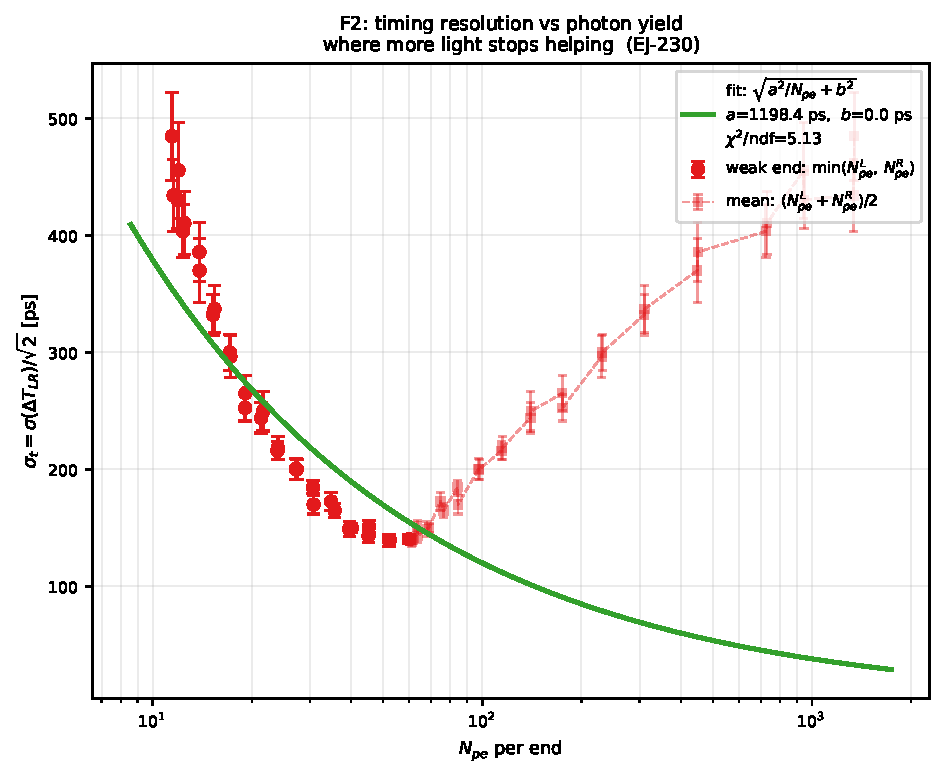
\includegraphics[width=0.90\textwidth,keepaspectratio]{fig02b.pdf}
    \end{column}
  \end{columns}
  \vspace{-0.35em}
  {\tiny
  \textbf{One position, two horizontal coordinates:}
  dark markers use $N_\text{weak}=\min(N_L,N_R)$ and are fitted; faint markers use
  $N_\text{mean}=(N_L+N_R)/2$ with the \emph{same} $\sigma_t$ and are not fitted.\\[-0.05em]
  For $x>0$, weak/far $=$ END\_LEFT; for $x<0$, weak/far $=$ END\_RIGHT; at $x=0$ they are equivalent.
  Thus a huge near-end signal can inflate $N_\text{mean}$ while the photon-starved far end still limits timing.\\[-0.05em]
  Fit: $\sigma_t=\sqrt{a^2/N_\text{weak}+b^2}$. Both fits place $b=0$ over
  $N_\text{weak}\in[11,77]$, but $\chi^2/\text{ndf}\simeq5$ means the
  $1/\sqrt{N_{pe}}$ description is approximate, not exact ``pure Poisson''.}
\end{frame}

\begin{frame}{F4: Top SiPM light yield vs position — \textbf{not} a timing quantity (EndTop EJ-204)}
  \centering
  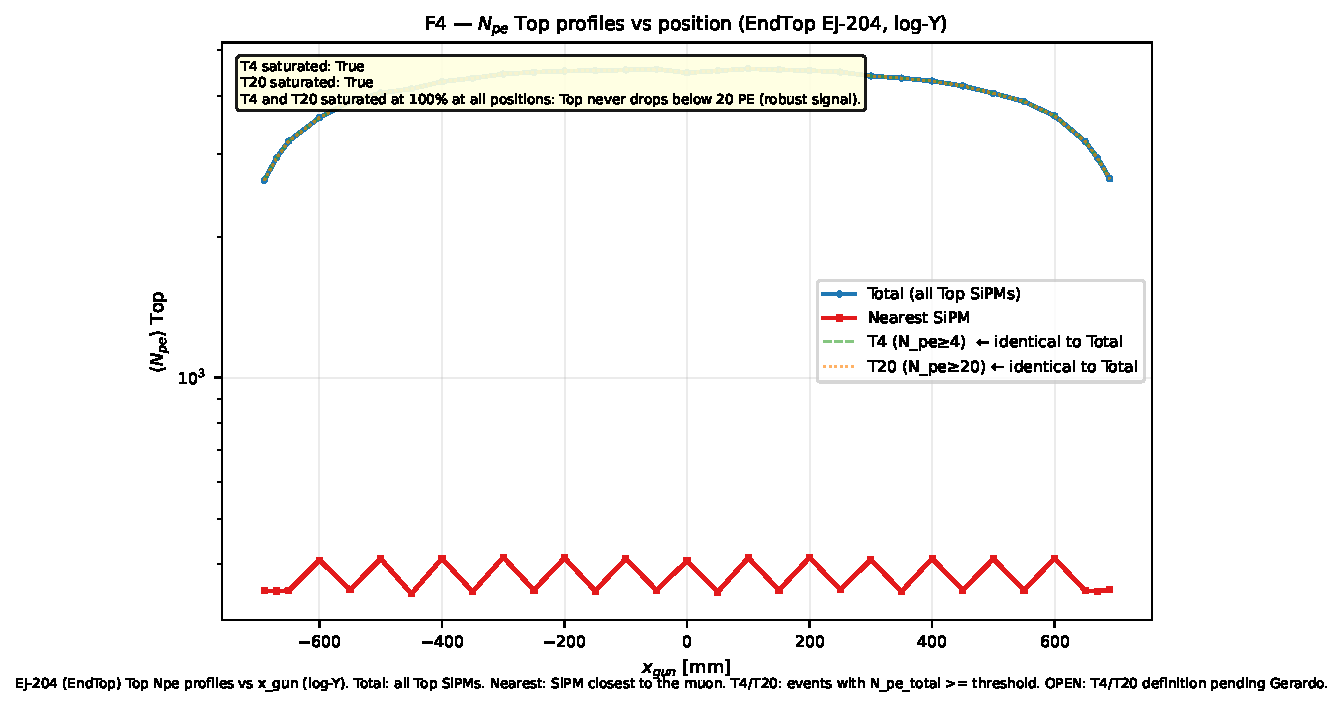
\includegraphics[width=0.59\textwidth,keepaspectratio]{fig04.pdf}

  \vspace{-0.3em}
  {\scriptsize
  \begin{itemize}\setlength\itemsep{0.05em}
    \item \textbf{TOP SiPMs} (IDs 16--85): Y-axis is light yield, not timing.
      ``Total'' sums all TOP channels; ``Nearest'' is the closest single channel and oscillates with the 20-mm pitch.
    \item All events pass the implemented T4/T20 selections, so those curves lie on Total:
      \textbf{100\% cut efficiency}, not electronic sensor saturation.
    \item {\color{pendgold}\textbf{Open — Gerardo:}}
      confirm whether T4/T20 are total-$N_{pe}$ cuts or a SUM4 trigger efficiency.
  \end{itemize}}
\end{frame}

% ══════════════════════════════════════════════════════════════════════════════
\section{Timing resolution SUM4 — F5}

\begin{frame}{F5: SUM4 L/R timing resolution — \textcolor{ej204col}{EJ-204}}
  \framesubtitle{$T_L$: END\_LEFT, $T_R$: END\_RIGHT, $\Delta T_{LR}=T_L-T_R$;
    width gives timing, peak position gives geometry}
  \centering
  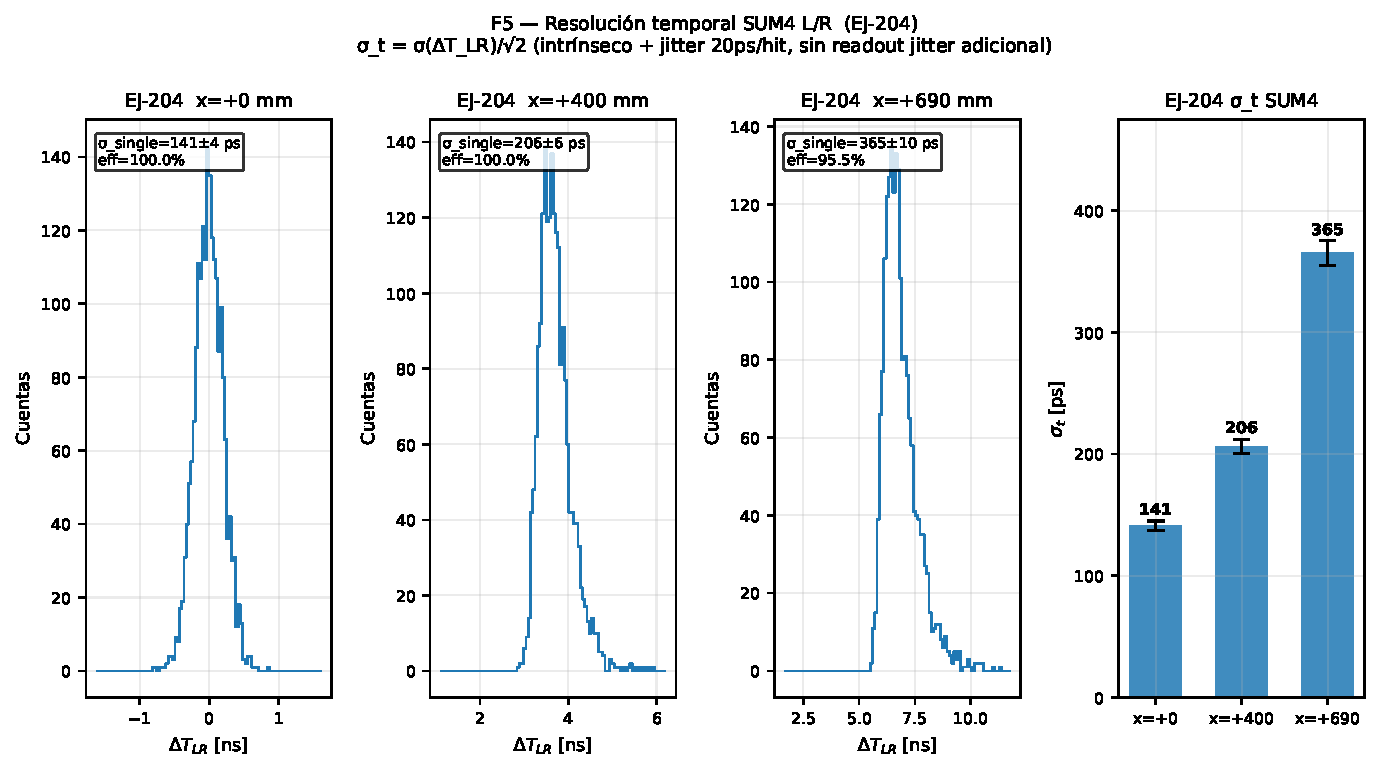
\includegraphics[width=0.70\textwidth,keepaspectratio]{fig05a.pdf}

  \vspace{-0.15em}
  {\scriptsize At $x>0$, END\_RIGHT is nearer, so $T_R<T_L$ and the peak moves to positive
  $\Delta T_{LR}$. The reported $\sigma_t=\sigma(\Delta T_{LR})/\sqrt{2}$ is an
  equivalent single-end benchmark; near the edge the two ends are not equally precise.
  Stage 1 reports the intrinsic timing resolution from photon counting and optical propagation,
  as produced directly by the simulation; no electronics or SiPM jitter is added.}
\end{frame}

\begin{frame}{F5: SUM4 L/R timing resolution — \textcolor{ej230col}{EJ-230}}
  \framesubtitle{$T_L$: END\_LEFT, $T_R$: END\_RIGHT, $\Delta T_{LR}=T_L-T_R$;
    stronger edge broadening and efficiency loss than EJ-204}
  \centering
  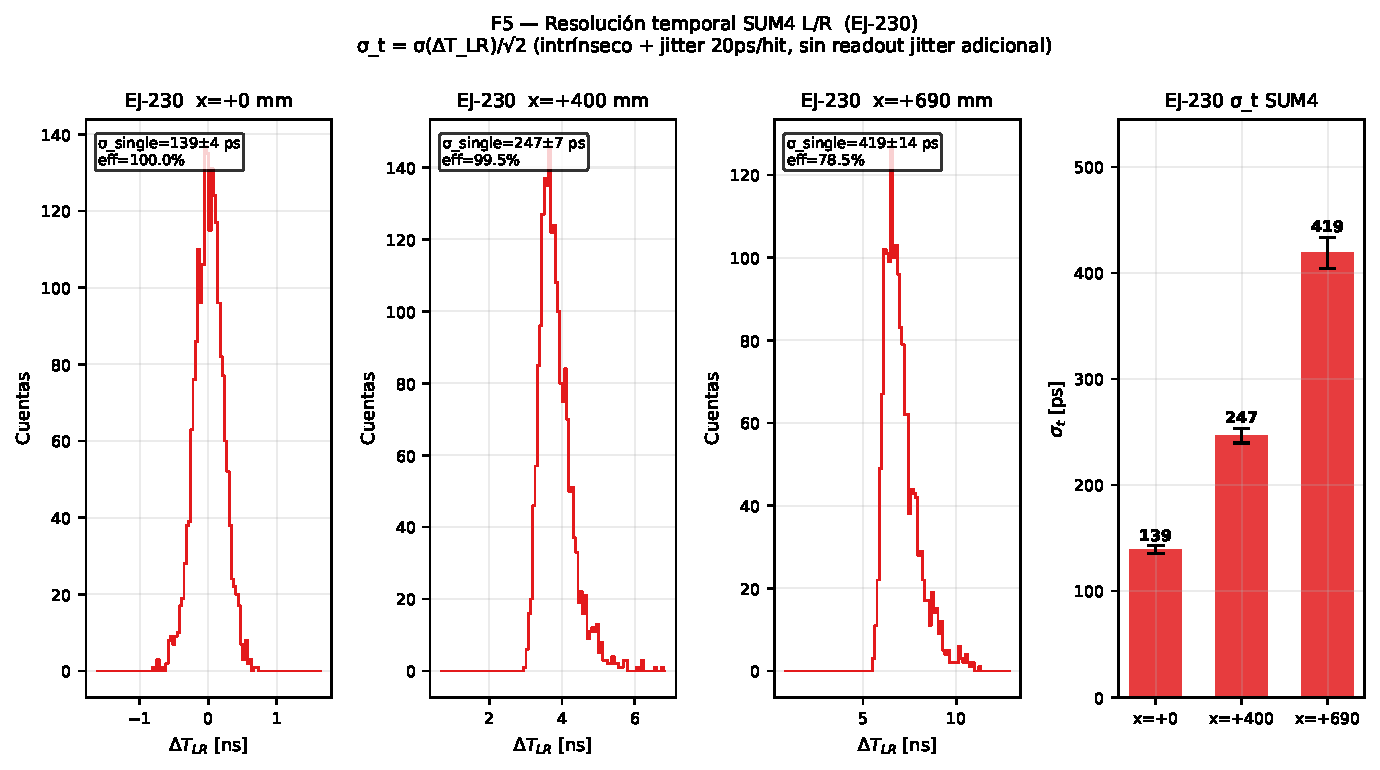
\includegraphics[width=0.70\textwidth,keepaspectratio]{fig05b.pdf}

  \vspace{-0.15em}
  {\scriptsize The peak shift with $x$ is the propagation-time asymmetry; the peak width and
  non-Gaussian tail quantify timing fluctuations. At $x=+690$\,mm the valid-event efficiency
  falls to 78.5\%, indicating that the far END\_LEFT often fails the SUM4 requirement.}
\end{frame}

\begin{frame}{Timing resolution comparison: EJ-204 vs EJ-230}
  \begin{center}
    \large
    \begin{tabular}{lrrr}
      \toprule
      Material & $x=0$\,mm & $x=+400$\,mm & $x=+690$\,mm \\
               & $\sigma_t$ [ps] & $\sigma_t$ [ps] & $\sigma_t$ [ps] \\
      \midrule
      \textcolor{ej204col}{\textbf{EJ-204}} & $141\pm4$ & $206\pm6$ & $365\pm10$ \\
      \textcolor{ej230col}{\textbf{EJ-230}} & $139\pm4$ & $247\pm7$ & $419\pm14$ \\
      \bottomrule
    \end{tabular}
  \end{center}
  \vspace{0.4em}
  \begin{columns}[T]
    \begin{column}{0.52\textwidth}
      \textbf{Key observations:}
      \begin{itemize}
        \item Central resolution \textbf{equivalent}: $141\approx139$\,ps
        \item At the edge, EJ-230 is $14.8\%$ larger than EJ-204
              ($419$ vs $365$\,ps; EJ-204 is $12.9\%$ lower if referenced to EJ-230)
        \item EJ-230 degrades faster with position\\
              ($+201\%$ vs $+159\%$ from $x=0$ to $x=690$)
        \item Fitted $\tau_f$: arrival-time profile (emission $\otimes$\ propagation)\\
              \textit{not} datasheet constants\\
              (EJ-204: $\tau_r^{(0)}=0.7$\,ns, $\tau_d^{(0)}=1.8$\,ns)
      \end{itemize}
    \end{column}
    \begin{column}{0.46\textwidth}
      {\small \color{gray}
      \textit{Caveats — Stage 1 (no real electronics):}
      \begin{itemize}
        \item Intrinsic simulation only: no electronics or SiPM jitter added
        \item No time-walk correction (ToT)
        \item $\sigma/\sqrt{2}$ is an equivalent metric; edge ends are asymmetric
        \item SUM4 (code-verified): fixed id$\,{/\!/}\,4$ clusters per end,
              earliest-of-two, leading-edge $\geq4$\,PE.
              Open: hardware fixed clusters vs moving-window.
        \item Recovering emission constants\\
              requires deconvolution — Stage 2
      \end{itemize}
      }
    \end{column}
  \end{columns}
\end{frame}

% ══════════════════════════════════════════════════════════════════════════════
\section{Top SiPM redundancy — F6}

\begin{frame}{F6: Top SiPM redundancy — $N_\text{pe}$ correlation between neighbors}
  \centering
  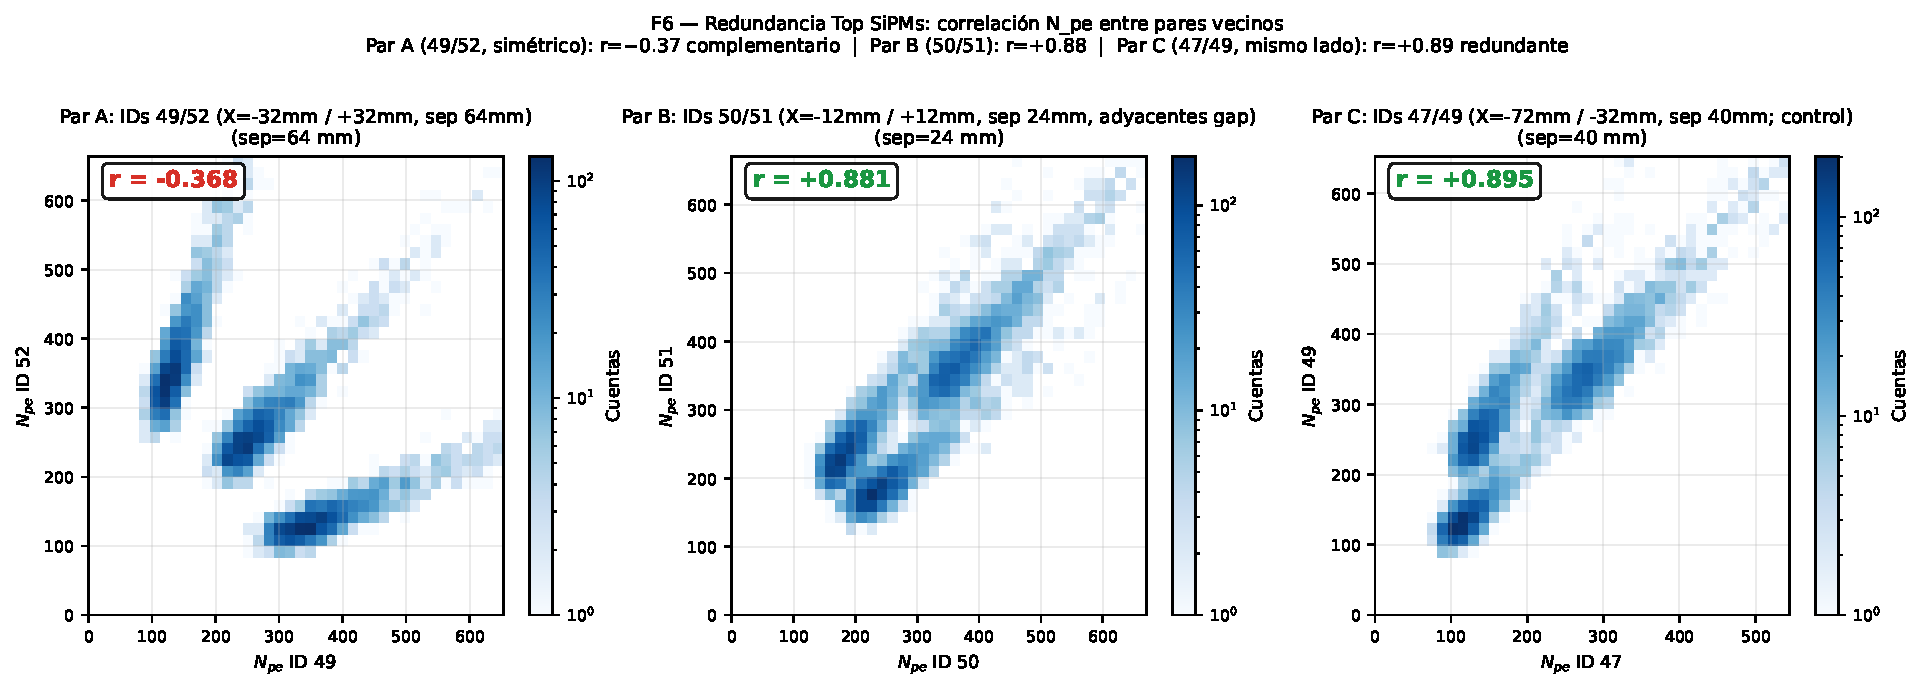
\includegraphics[width=0.78\textwidth,keepaspectratio]{fig06.pdf}

  \vspace{-0.15em}
  {\footnotesize\begin{columns}[T]
    \begin{column}{0.32\textwidth}
      \centering
      \textbf{Pair A (IDs 49/52)}\\
      sep $=64$\,mm, opposite sides\\
      $r=-0.37$ — complementary\\
      {\footnotesize (light splits between sides)}
    \end{column}
    \begin{column}{0.32\textwidth}
      \centering
      \textbf{Pair B (IDs 50/51)}\\
      sep $=24$\,mm, across gap\\
      $r=+0.88$ — \textbf{strongly correlated}\\
      {\footnotesize (same light source)}
    \end{column}
    \begin{column}{0.32\textwidth}
      \centering
      \textbf{Pair C (IDs 47/49)}\\
      sep $=40$\,mm, same side\\
      $r=+0.90$ — \textbf{strongly correlated control}\\
      {\footnotesize (local correlation expected)}
    \end{column}
  \end{columns}}
  \vspace{-0.1em}
  \begin{center}
    {\tiny Pearson $r$ measures linear correlation only. High pooled $r$ marks a candidate
    redundancy, not proof that a channel can be removed; fixed-position trigger/reconstruction tests are required.}
  \end{center}
\end{frame}

% ══════════════════════════════════════════════════════════════════════════════
\section{Optical path dispersion — F7}

\begin{frame}{F7: Order-statistic arrival time $\langle t_n\rangle$ per Top channel —
              $x=-690$\,mm}
  \framesubtitle{Observed RMS vs idealized order-statistics floor
    $\sigma_\text{stat}(t_n)\simeq\sqrt{n}\,\tau_d/\langle N_\text{pe}\rangle$}
  \begin{columns}[c]
    \begin{column}{0.59\textwidth}
      \centering
      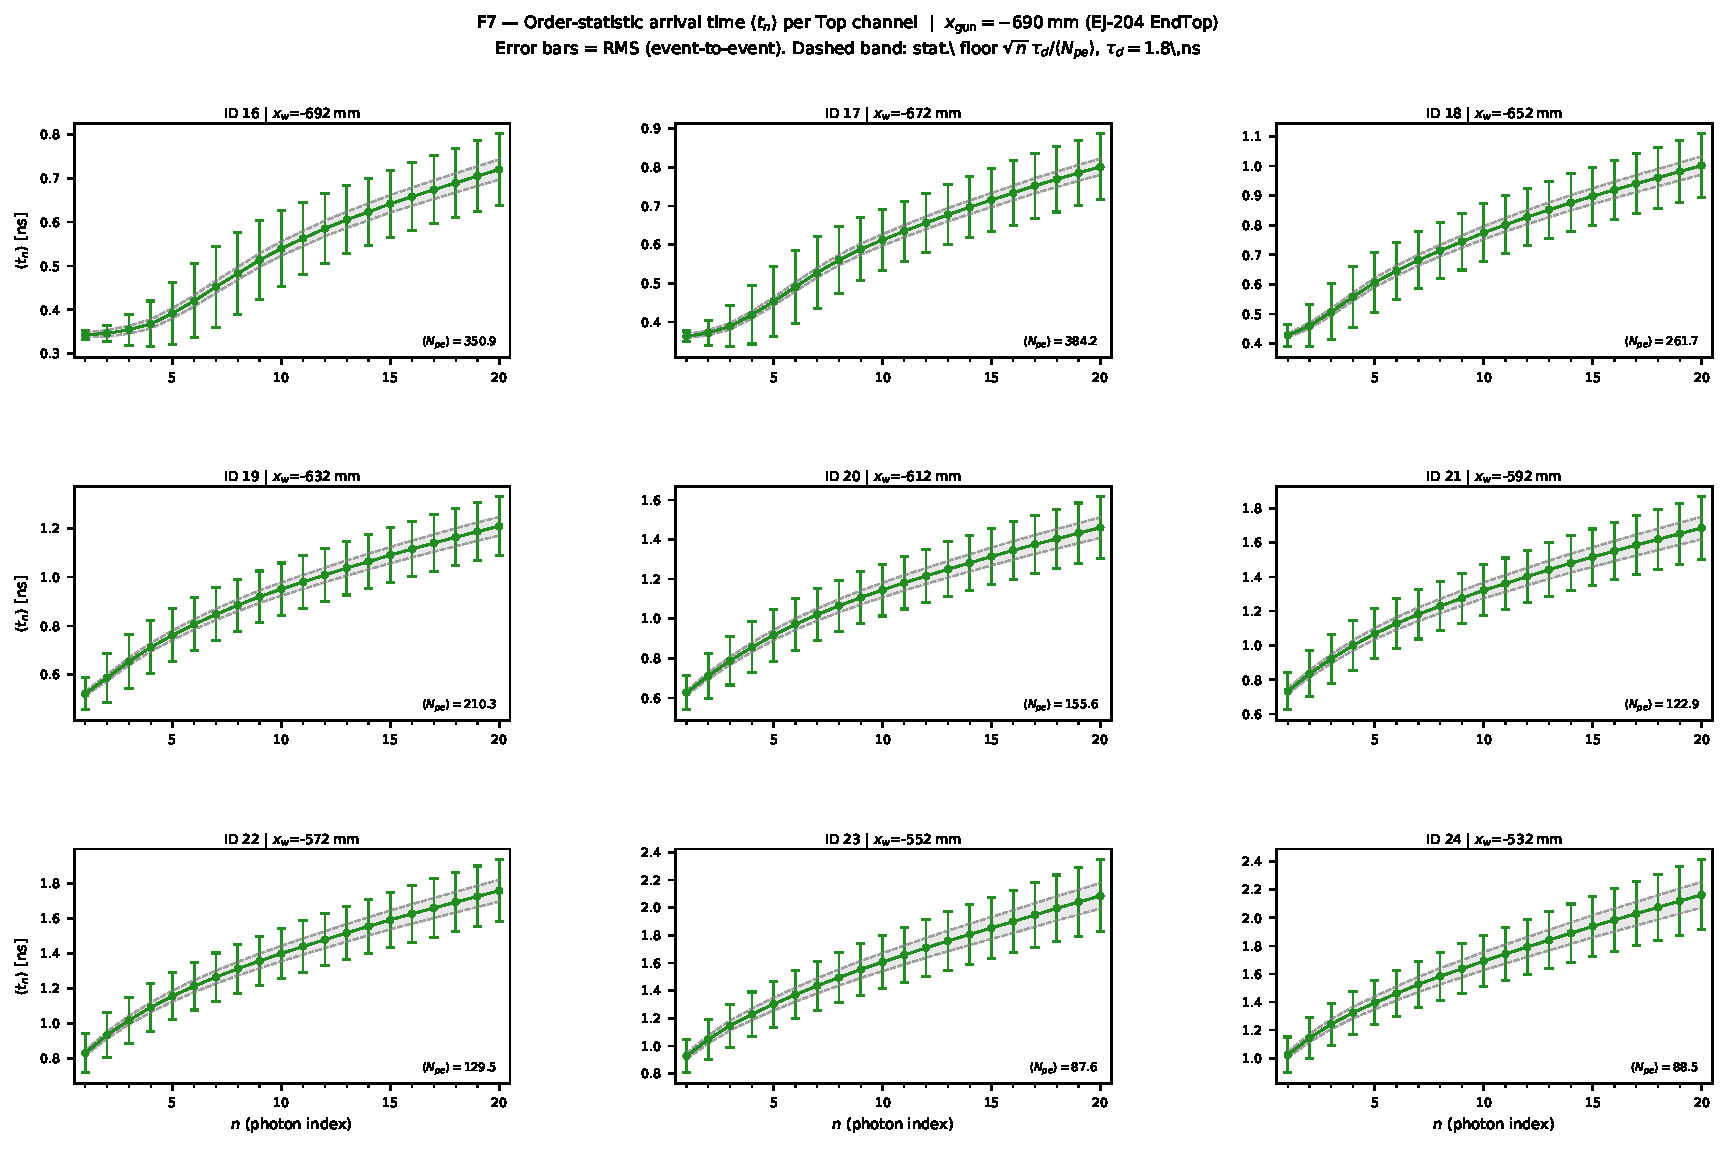
\includegraphics[width=\textwidth,keepaspectratio]{fig07.pdf}
    \end{column}
    \begin{column}{0.39\textwidth}
      \textbf{How to read it:}
      \begin{itemize}\setlength\itemsep{0.15em}
        \item $n$: index of the $n$-th detected photon in one event/channel.
        \item $\langle t_n\rangle$: mean arrival time; it rises with $n$ by construction.
        \item Error bars: event-to-event RMS, \textbf{not} uncertainty on the mean.
        \item Dashed band: idealized statistical floor using $\tau_d=1.8$\,ns.
      \end{itemize}
      \vspace{0.1em}
      {\footnotesize
      RMS above the floor indicates an additional contribution compatible with optical-path
      dispersion. Widths must not be subtracted linearly; if independent,
      \[
        \sigma_\text{extra}\simeq
        \sqrt{\sigma_\text{obs}^2-\sigma_\text{stat}^2}.
      \]
      IDs 16--24 span $x_w=-692\to-532$\,mm and are truncated by the left edge.
      The connection to F2 is qualitative: F7 uses TOP channels, whereas F2 uses END timing.}
    \end{column}
  \end{columns}
\end{frame}

% ══════════════════════════════════════════════════════════════════════════════
\section{Summary}

\begin{frame}{Summary and open questions}
  \footnotesize
  \begin{columns}[T]
    \begin{column}{0.54\textwidth}
      \textbf{Main results:}
      \begin{enumerate}
        \item \textcolor{ej204col}{\textbf{EJ-204}} $\approx$
              \textcolor{ej230col}{\textbf{EJ-230}} at center ($141$ vs $139$\,ps);
              EJ-204 \textbf{better at edges} ($365$ vs $419$\,ps at $x=690$)

        \item F1 component at $\sim4.7$\,ns at $x=690$ =
              \textcolor{okgreen}{\textbf{geometric ToF}} from far end
              (QA-1c, $\delta=-5\%$). Not slow scintillation.

        \item $v_\text{eff}^\text{nominal}=277$\,mm/ns;
              onset gives $v_\text{eff}^\text{onset}\approx292$\,mm/ns ($+5\%$)
              — fastest optical paths set the onset

        \item F2: timing follows a photon-statistics-dominated trend versus the weak end;
              no nonzero constant floor is resolved, although the simple fit has $\chi^2/\text{ndf}\sim5$

        \item F7: the observed $t_n$ RMS exceeds an idealized statistical floor;
              the excess is evidence for an additional contribution compatible with
              optical-path dispersion (quadrature subtraction is required)

        \item Top: all events pass the implemented 20-PE cut; gap-adjacent SiPMs
              are strongly correlated ($r\approx0.88$), a candidate redundancy
      \end{enumerate}
    \end{column}
    \begin{column}{0.44\textwidth}
      \textbf{\color{pendgold} Open — Gerardo confirmation:}
      \begin{itemize}
        \item[$\boxtimes$] SUM4 (code-verified): fixed id$/\!/$4 clusters,
              earliest-of-two, leading-edge $\geq4$\,PE.
              Open: hardware fixed vs moving-window.
        \item[$\square$] T4/T20: $N_\text{pe}$ cut or trigger efficiency
        \item[$\boxtimes$] Jitter: intrinsic simulation used as-is;
              no electronics or SiPM jitter term added.
        \item[$\square$] F3: SiPM impacts vs volume trajectories
        \item[$\square$] Pair A ($r=-0.37$):
              geometric or reflections
        \item[$\square$] EJ-230 tail at $x=0$:
              slow mode or reflections?
      \end{itemize}
      \vspace{0.05em}
      \textbf{Next steps:}
      \begin{itemize}
        \item EJ-230 EndTop dataset (Top response)
        \item Stage 2: time-walk, readout jitter, real electronics
        \item Deconvolution: emission constants from arrival profiles
      \end{itemize}
    \end{column}
  \end{columns}
\end{frame}

\end{document}
